
\documentclass{beamer}
\usepackage[latin1]{inputenc}
%\usetheme{Montpellier}
%\usetheme{Boadilla}
%\usecolortheme[RGB={204,51,255}]{structure}
%\usecolortheme[named=purple]{structure}
\usecolortheme[RGB={62,128,62}]{structure}
%\definecolor{reddish}{rgb}{0.3,0.15,0.3}
%\definecolor{light}{rgb}{0.8,0.6,0.8}
%\definecolor{reddish}{rgb}{.5,0.15,0.15}
\definecolor{reddish}{rgb}{0.5,0.3,0.4}
%\definecolor{light}{rgb}{0.8,0.6,0.8}
\definecolor{reddish}{rgb}{.7,0.25,0.25}
\definecolor{greenish}{rgb}{.25,0.8,0.25}
\definecolor{blueish}{rgb}{.25,0.25,0.7}
\definecolor{purple}{rgb}{.5,0.0,0.5}
\usepackage{graphicx}
\usepackage{pstricks}
\usepackage{epsfig}
\newcommand{\btVFill}{\vskip0pt plus 1filll}

\setbeamertemplate{navigation symbols}{}

\newcommand{\crish}{\color{reddish}}
\newcommand{\cgish}{\color{greenish}}
\newcommand{\cbla}{\color{black}}
\newcommand{\cred}{\color{red}}
\newcommand{\cblu}{\color{blue}}
\newcommand{\cgrish}{\color{green}}

\newcommand{\sm}{\color{reddish}$}
\newcommand{\fm}{$\color{black}{}}

\newcommand{\letter}[1]{\color{blue}\texttt{#1}\color{black}}
\newcommand{\binary}[1]{\color{red}\texttt{#1}\color{black}}

\usepackage{tikz}
\usetikzlibrary{arrows,decorations.markings,positioning}
\usepackage{epstopdf}
\usetikzlibrary{fit}
\usepackage{pgfplots}

\title[Information Theory lecture 11]{Infomax: information theory lecture 11}
\author{COMSM0075 Information Processing and Brain}
\institute{\texttt{comsm0075.github.io}}
\date{October 2020}

\begin{document}

\maketitle

\begin{frame}{Source separation}
  \cred
  $$
 \mathbf{ s}\stackrel{\mbox{mixing}}{\longrightarrow}\mathbf{r}=M\mathbf{ s}\stackrel{\mbox{unmixing}}{\longrightarrow}\mathbf{ x}=W\mathbf{r}
 $$
 \cbla
\end{frame}

\begin{frame}{Mutual information}
    \cred
  $$
 \mathbf{ s}\stackrel{\mbox{mixing}}{\longrightarrow}\mathbf{r}=M\mathbf{ s}\stackrel{\mbox{unmixing}}{\longrightarrow}\mathbf{ x}=W\mathbf{r}
 $$
 \cbla
  Two-dimensional case: we are assuming the two sources \crish$S_1$\cbla{} and \crish$S_2$\cbla{} are independent, so we want to find independent \crish$X_1$\cbla{} and \crish$X_2$\cbla.
\end{frame}

\begin{frame}{Mutual information}
  \crish $$\textbf{X}=W\textbf{R}$$\cbla
  Two-dimensional case: we are assuming the two sources \crish$S_1$\cbla{} and \crish$S_2$\cbla{} are independent, so we want to find independent \crish$X_1$\cbla{} and \crish$X_2$\cbla:
  \crish
  $$
  I(X_1,X_2)=0
  $$
  \cbla
  or at the very least we'll try to minimize \cblu$I(X_1,X_2)$\cbla{}.
\end{frame}


\begin{frame}{Infomax}
  We want to minimize \cblu$I(X_1,X_2)$\cbla{} but this is very hard to calculate!
  \crish
  $$
  I(X_1,X_2)=h(X_1)+h(X_2)-h(X_1,X_2)
  $$
  \cbla
  Let's maximize \crish$h(X_1,X_2)$\cbla{} instead.
  
\end{frame}


\begin{frame}{Infomax}
  We want to minimize $I(X_1,X_2)$\cbla{} but this is very hard to calculate!
  \crish
  $$
  I(X_1,X_2)=h(X_1)+h(X_2)-h(X_1,X_2)
  $$
  \cbla
  Let's \cblu{}maximize $h(X_1,X_2)$\cbla{} instead: \cblu{}Infomax\cbla{}.
  \end{frame}



\begin{frame}{Infomax}
  We want to minimize $I(X_1,X_2)$\cbla{} but this is very hard to calculate!
  \crish
  $$
  I(X_1,X_2)=h(X_1)+h(X_2)-h(X_1,X_2)
  $$
  \cbla
  Let's maximize \crish$h(X_1,X_2)$\cbla{} instead.
  \begin{itemize}
  \item This means ignoring \crish$h(X_1)$\cbla{} and \crish$h(X_2)$\cbla{}.
  \item It isn't obvious \crish$h(X_1,X_2)$\cbla{} is any easier to calculate than \crish$I(X_1,X_2)$\cbla{}.
  \end{itemize}
\end{frame}

\begin{frame}{An obvious problem}
  The differential entropy isn't scale invariant
  \crish
  $$
  h(\cblu{}\lambda\crish{}{}X_1,X_2)=h(X_1,X_2)+\log_2{|\cblu{}\lambda\crish{}|}
  $$
  \cbla
  so it tells us nothing about mixing and unmixing.
  \end{frame}


\begin{frame}{An obvious problem}
  The differential entropy isn't scale invariant
  \crish
  $$
  h(X_1,\cblu{}\lambda\crish{}{}X_2)=h(X_1,X_2)+\log_2{|\cblu{}\lambda\crish{}|}
  $$
  \cbla
    so it tells us nothing about mixing and unmixing.
  \end{frame}

\begin{frame}{An obvious problem}
  The differential entropy isn't scale invariant
  \crish
  $$
  h(\cblu{}\lambda\crish{}{}X_1,\cblu{}\lambda\crish{}{}X_2)=h(X_1,X_2)+2\log_2{|\cblu{}\lambda\crish{}|}
  $$
  \cbla
    so it tells us nothing about mixing and unmixing.
\end{frame}

\begin{frame}{A very clever solution}
  Inspire by the behaviour of neurons Bell and Sejnowski added a saturating non-linearity:
  \crish
  \begin{eqnarray*}
y_1&=&g(x_1+w_1)\cr
y_2&=&g(x_2+w_2)
\end{eqnarray*}
  \cbla
  where  \crish$w_1$\cbla{} and \crish$w_2$\cbla{} are parameters and, for example,
\crish $$
g(u)=\frac{1}{1+e^{-u}}
$$ \cbla{}
is a saturating non-linearity so \crish$g:(-\infty,\infty)\rightarrow (0,1)$.\cbla{}
  \vfill
  \flushright{\tiny{Bell, A. J. and Sejnowski, T. J. (1995)}}
\end{frame}


\begin{frame}{Saturating non-linearity}

\crish $$
g(u)=\frac{1}{1+e^{-u}}
$$ \cbla{}
is a saturating non-linearity so \crish$g:(-\infty,\infty)\rightarrow (0,1)$.\cbla{}
\begin{center}
  \epsfig{file=g.eps,width=4cm,angle=270}
\end{center}
\end{frame}

\begin{frame}{Saturating non-linearity}
  Say \crish$X$\cbla{} is uniform
    \cbla
  \begin{center}
    \begin{tikzpicture}
    \node[](left){$\ldots$};
    \node[right =  1cm of left](zero){};
    \node[above = 2cm of zero](overzero){};
    \node[right = 0.5cm of overzero](overa){};
    \node[below = 2cm of overa](a){};
    \node[right = 1cm of a](right){$\ldots$};
    \draw[thick] (left) -- (zero.center) -- (overzero.center) -- (overa.center) -- (a.center) -- (right);
    \draw[dotted] (zero.center) -- (a.center);
    \node[below = 0.01 cm of zero.west](belowzero){$-\frac{a}{2}$};
    \node[below = 0.01 cm of a.center](belowa){$\frac{a}{2}$};
    \node[left = 0.0675 cm of overzero](leftoverzero){$\frac{1}{a}$};
    \end{tikzpicture}
  \end{center}
  \end{frame}


\begin{frame}{Saturating non-linearity}
  Now calculate \crish
  $$
  p_G(g) = \frac{p_X(x(g))}{dg/dx}
  $$
  \cbla{}
\end{frame}


\begin{frame}{Saturating non-linearity}
  Now calculate \crish$p_G(g)$\cbla{}
\begin{center}
  % GNUPLOT: LaTeX picture with Postscript
\begingroup
  \makeatletter
  \providecommand\color[2][]{%
    \GenericError{(gnuplot) \space\space\space\@spaces}{%
      Package color not loaded in conjunction with
      terminal option `colourtext'%
    }{See the gnuplot documentation for explanation.%
    }{Either use 'blacktext' in gnuplot or load the package
      color.sty in LaTeX.}%
    \renewcommand\color[2][]{}%
  }%
  \providecommand\includegraphics[2][]{%
    \GenericError{(gnuplot) \space\space\space\@spaces}{%
      Package graphicx or graphics not loaded%
    }{See the gnuplot documentation for explanation.%
    }{The gnuplot epslatex terminal needs graphicx.sty or graphics.sty.}%
    \renewcommand\includegraphics[2][]{}%
  }%
  \providecommand\rotatebox[2]{#2}%
  \@ifundefined{ifGPcolor}{%
    \newif\ifGPcolor
    \GPcolorfalse
  }{}%
  \@ifundefined{ifGPblacktext}{%
    \newif\ifGPblacktext
    \GPblacktexttrue
  }{}%
  % define a \g@addto@macro without @ in the name:
  \let\gplgaddtomacro\g@addto@macro
  % define empty templates for all commands taking text:
  \gdef\gplbacktext{}%
  \gdef\gplfronttext{}%
  \makeatother
  \ifGPblacktext
    % no textcolor at all
    \def\colorrgb#1{}%
    \def\colorgray#1{}%
  \else
    % gray or color?
    \ifGPcolor
      \def\colorrgb#1{\color[rgb]{#1}}%
      \def\colorgray#1{\color[gray]{#1}}%
      \expandafter\def\csname LTw\endcsname{\color{white}}%
      \expandafter\def\csname LTb\endcsname{\color{black}}%
      \expandafter\def\csname LTa\endcsname{\color{black}}%
      \expandafter\def\csname LT0\endcsname{\color[rgb]{1,0,0}}%
      \expandafter\def\csname LT1\endcsname{\color[rgb]{0,1,0}}%
      \expandafter\def\csname LT2\endcsname{\color[rgb]{0,0,1}}%
      \expandafter\def\csname LT3\endcsname{\color[rgb]{1,0,1}}%
      \expandafter\def\csname LT4\endcsname{\color[rgb]{0,1,1}}%
      \expandafter\def\csname LT5\endcsname{\color[rgb]{1,1,0}}%
      \expandafter\def\csname LT6\endcsname{\color[rgb]{0,0,0}}%
      \expandafter\def\csname LT7\endcsname{\color[rgb]{1,0.3,0}}%
      \expandafter\def\csname LT8\endcsname{\color[rgb]{0.5,0.5,0.5}}%
    \else
      % gray
      \def\colorrgb#1{\color{black}}%
      \def\colorgray#1{\color[gray]{#1}}%
      \expandafter\def\csname LTw\endcsname{\color{white}}%
      \expandafter\def\csname LTb\endcsname{\color{black}}%
      \expandafter\def\csname LTa\endcsname{\color{black}}%
      \expandafter\def\csname LT0\endcsname{\color{black}}%
      \expandafter\def\csname LT1\endcsname{\color{black}}%
      \expandafter\def\csname LT2\endcsname{\color{black}}%
      \expandafter\def\csname LT3\endcsname{\color{black}}%
      \expandafter\def\csname LT4\endcsname{\color{black}}%
      \expandafter\def\csname LT5\endcsname{\color{black}}%
      \expandafter\def\csname LT6\endcsname{\color{black}}%
      \expandafter\def\csname LT7\endcsname{\color{black}}%
      \expandafter\def\csname LT8\endcsname{\color{black}}%
    \fi
  \fi
    \setlength{\unitlength}{0.0500bp}%
    \ifx\gptboxheight\undefined%
      \newlength{\gptboxheight}%
      \newlength{\gptboxwidth}%
      \newsavebox{\gptboxtext}%
    \fi%
    \setlength{\fboxrule}{0.5pt}%
    \setlength{\fboxsep}{1pt}%
\begin{picture}(4320.00,3024.00)%
    \gplgaddtomacro\gplbacktext{%
      \csname LTb\endcsname%%
      \put(462,440){\makebox(0,0)[r]{\strut{}$0$}}%
      \put(462,1225){\makebox(0,0)[r]{\strut{}$5$}}%
      \put(462,2011){\makebox(0,0)[r]{\strut{}$10$}}%
      \put(462,2796){\makebox(0,0)[r]{\strut{}$15$}}%
      \put(594,220){\makebox(0,0){\strut{}$0$}}%
      \put(1260,220){\makebox(0,0){\strut{}$0.2$}}%
      \put(1926,220){\makebox(0,0){\strut{}$0.4$}}%
      \put(2591,220){\makebox(0,0){\strut{}$0.6$}}%
      \put(3257,220){\makebox(0,0){\strut{}$0.8$}}%
      \put(3923,220){\makebox(0,0){\strut{}$1$}}%
    }%
    \gplgaddtomacro\gplfronttext{%
      \csname LTb\endcsname%%
      \put(2936,2630){\makebox(0,0)[r]{\strut{}$a=1$}}%
      \csname LTb\endcsname%%
      \put(2936,2410){\makebox(0,0)[r]{\strut{}$a=5$}}%
      \csname LTb\endcsname%%
      \put(2936,2190){\makebox(0,0)[r]{\strut{}$a=10$}}%
    }%
    \gplbacktext
    \put(0,0){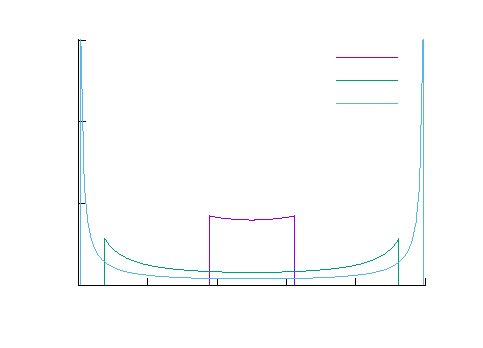
\includegraphics{g_output}}%
    \gplfronttext
  \end{picture}%
\endgroup

  \end{center}
\end{frame}


\begin{frame}{Saturating non-linearity}
  Now calculate \crish$p_G(g)$\cbla{}
\begin{center}
  \begin{tabular}{ll}
    $a=1$&$h(G)=-1.41$\\
    $a=5$&$h(G)=-0.26$\\
    $a=10$&$h(G)=-1.03$\\
    $a=15$&$h(G)=-11.6$
    \end{tabular}
  \end{center}

\end{frame}


\begin{frame}{Unmixing}
\cred
$$
\mathbf{ s}\stackrel{\mbox{mixing}}{\longrightarrow}\mathbf{ r}=M\mathbf{ s}\stackrel{\mbox{unmixing}}{\longrightarrow}\mathbf{ x}=W\mathbf{ r}\stackrel{\mbox{non-linearity}}{\longrightarrow}\mathbf{y}=g.(\mathbf{x}+\mathbf{w})
$$
\cbla
using the broadcast notation \crish$$g\cblu.\crish(\mathbf{x}+\mathbf{w})=(g(x_1+w_1),g(x_2+w_2))$$\cbla
\end{frame}


\begin{frame}{Unmixing}
\cred
$$
\mathbf{ s}\stackrel{\mbox{mixing}}{\longrightarrow}\mathbf{ r}=M\mathbf{ s}\stackrel{\mbox{unmixing}}{\longrightarrow}\mathbf{ x}=W\mathbf{ r}\stackrel{\mbox{non-linearity}}{\longrightarrow}\mathbf{y}=g.(\mathbf{x}+\mathbf{w})
$$
\cbla
For later convenience:
\crish
$$
\mathbf{y}=g.(\mathbf{x}+\mathbf{w})=\mathbf{f}(\mathbf{r};W,\mathbf{w})
$$
\cbla
\end{frame}

\begin{frame}{One-dimensional problem}
  \cred
$$
r\stackrel{\mbox{multiply}}{\longrightarrow}x=Wr\stackrel{\mbox{non-linearity}}{\longrightarrow}y=g(x+w)=f(r;w,W)
$$\cbla
where \crish$W$\cbla{} and \crish$w$\cbla{} are both scalars. We want to maximize the entropy \cblu$h(Y)$\cbla{}, this should also maximize the information in \crish$Y$\cbla{} about \crish$R$\cbla:
\crish $$
I(R;Y)=h(Y)-h(Y|R)
$$\cbla
but \crish$h(Y|R)$\cbla{} is constant since \crish$R$\cbla{} determines \crish$Y$\cbla.
\end{frame}


\begin{frame}{Don't panic}

\crish $$
I(R;Y)=h(Y)-h(Y|R)
$$\cbla and \crish$h(Y|R)$\cbla{} is constant since \crish$R$\cbla{}
determines \crish$Y$\cbla. For differential entropy the constant is
minus infinity not zero as it would be for discrete entropy, but since
we are interested in derivative all that counts is that it's a constant!
\end{frame}


\begin{frame}{Estimating $h(Y)$}
  As we know
  \crish$$
h(Y)=-\int p(y)\log{p(y)} dy
$$\cbla
and this is estimated by
\crish$$
\tilde{h}(y)=-\log{p(y)}
$$\cbla
meaning if \crish$n$\cbla{} values \crish$y^t$\cbla{} are drawn from \crish$Y$\cbla{} then
\crish
$$
\frac{1}{n}\sum_t\tilde{h}(y^t)\rightarrow h(Y)
$$
\cbla
as \crish$n$\cbla{} gets large. 
\end{frame}

\begin{frame}{We don't need $p_Y(y)$}
  The plan is to maximize \crish$h(Y)$\cbla{} by gradient ascent.
  \vskip 2cm
\begin{center}
  \includegraphics[width=11cm]{Pendle.jpg}
\end{center}
\vfill
\flushright{\tiny{Picture of Pendle from Wikipedia}}
\end{frame}


\begin{frame}{We don't need $p_Y(y)$}
We can't estimate \crish$h(Y)$\cbla{} because we don't have $p_Y(y)$,
but it turns out we can still calculate the derivative.
\crish
$$
p_Y(y)=\frac{p_R[r=f^{-1}(y)]}{|f'(f^{-1}(y)|}
$$
\cbla{}
so \crish
$$
\tilde{h}(y)=\tilde{h}(r)+\log{|f'|}
$$
\cbla
and \crish$p_R(r)$\cbla{} is independent of the parameters.
\end{frame}

\begin{frame}{We can do the calculation}
  \cblu{}We want $dh/dW$ and $dh/dw$.\cbla{}
  \crish
  \begin{eqnarray*}
g(u)&=&\frac{1}{1+\exp{(-u)}}\cr
\frac{dg}{du}&=&g(1-g)
  \end{eqnarray*}
  \cbla
  and hence
  \crish
$$
\log{|f'|}=\log{W}+\log{f}+\log{(1-f)}
$$
\cbla{}
\end{frame}

\begin{frame}{We continue doing the calculation}
  \crish$$
f=g(Wr+w)
$$\cbla{}
so
\crish$$
\frac{df}{dW}=rf(1-f)
$$\cbla{}
and hence, 
\crish$$
\frac{d\tilde{h}(y)}{dW}=\frac{1}{W}+\frac{1}{f}rf(1-f)-\frac{1}{1-f}rf(1-f)=\frac{1}{W}+r(1-2y)
$$\cbla{}
Similarly
\crish$$
\frac{d\tilde{h}(y)}{dw}=1-2y
$$\cbla{}
\end{frame}


\begin{frame}{This is all stuff we know}
\crish$$
\frac{d\tilde{h}(y)}{dW}=\frac{1}{W}+r(1-2y)
$$\cbla{}
and
\crish$$
\frac{d\tilde{h}(y)}{dw}=1-2y
$$\cbla{}\crish$r$\cbla{} is the recorded value which we can sample;
\crish$W$\cbla{} and \crish$w$\cbla{} are the variables we want to
work out.
\end{frame}

\begin{frame}{We can do hill-climbing}
If we have the derivatives we can use an hill-climbing algorithm
like steepest ascent, conjugate gradient or metric gradient; the
latter works particularly well here.
\end{frame}

\begin{frame}{Example}
  Initial distribution \cblu$p_R(r)$\cbla:
  \begin{center}
    \epsfig{file=pr.eps,width=5cm,angle=270}
  \end{center}
\end{frame}

\begin{frame}{Example}
  After \crish$u=Wr+w$\cbla{} we have \cblu$p_U(u)$\cbla:
  \begin{center}
    \epsfig{file=pu.eps,width=5cm,angle=270}
  \end{center}
\end{frame}
  

\begin{frame}{Example}
  The non-linearity give \crish$y=g(Wr+w)$\cbla{} we have \cblu$p_Y(y)$\cbla:
  \begin{center}
    \epsfig{file=y.eps,width=5cm,angle=270}
  \end{center}
\end{frame}


\begin{frame}{Back to the $2\times2$ case}
\cred
$$
\mathbf{ s}\stackrel{\mbox{mixing}}{\longrightarrow}\mathbf{ r}=M\mathbf{ s}\stackrel{\mbox{unmixing}}{\longrightarrow}\mathbf{ x}=W\mathbf{ r}\stackrel{\mbox{non-linearity}}{\longrightarrow}\mathbf{y}=g.(\mathbf{x}+\mathbf{w})
$$
\cbla
A similar calculation gives
\crish
\begin{eqnarray*}
\frac{d\tilde{h}(\mathbf{y})}{dW_{ab}}&=&(W^T)^{-1}_{ab}+r_a(1-2y_b)\cr
\frac{d\tilde{h}(\mathbf{y})}{dw_a}&=&1-2y_a
\end{eqnarray*}
\cbla
allowing use to maximize \crish$h(Y_1,Y_2)$\cbla{}. This is Infomax!
\end{frame}
\end{document}

